\chapter{Metodologia}
\label{chap:metodologia}

Um dos pontos característico do programa de Formação em Robótica é a sua metodologia, onde buscará a aprendizagem ativa do estudante, com a construção dos seus conhecimentos, complementando as aulas expositivas com atividades e dinâmicas de grupo, elaboração e apresentação de trabalhos e pesquisas, emprego de meios audiovisuais, estudos individualizados, pesquisa de artigos técnicos e científicos, entre outros condicionantes ao programa.
A metodologia em si é um caminho para o sucesso na formação dos estudantes, pois esta convergência baseia-se em 5 pontos principais:

\begin{enumerate}
    \item \textbf{Criatividade:} espaço que estimula a criatividade, possibilitando interação e acesso à diferentes tecnologias.
    \item \textbf{Engajamento:} atividades práticas de aprendizado aumentam os níveis de concentração
    \item \textbf{Programação:} a inteligência artificial se torna cada vez mais presente nas escolas e escritórios
    \item \textbf{Trabalho em equipe:} robótica incorpora uma gama de habilidades e promove um ambiente de aprendizagem para pessoas com diferentes talentos
    \item \textbf{Diversão:} aprender sobre robótica deve ser divertido, e a medida que os estudantes continuem melhorando sua interação com eles, isso aumenta mais ainda o nível de diversão
\end{enumerate}


Basicamente o caminho para o sucesso compreende em 4 fases distintas, demonstradas na Figura \ref{fig:metodologia}:

\textbf{Assimilação:} desenvolver habilidades de codificação e lógica;

\textbf{Simulação:} testar as missões de um robô de forma eficiente;

\textbf{Integração:} garantir informações sobre o ambiente e o robô;

\textbf{Criação:} elaborar um projeto aplicado a tecnologia.

As três primeiras fases são compreendidas em 6 meses, ficando a fase Criação com 6 meses para finalizar o programa.
Entre cada fase, desafios são lançados para que o estudante obtenha maior sucesso na assimilação dos conceitos ministrados, para a última fase um projeto final é lançado para que o estudante possa realizar a demonstração de seu sistema para os avaliadores.
Bom salientar que durante as fases, temas serão tratados e discutidos de forma expositiva e prática.


\begin{figure}[H]
    \caption{Metodologia do Programa de Formação em Robótica e Sistemas Autônomos}
    \centering
    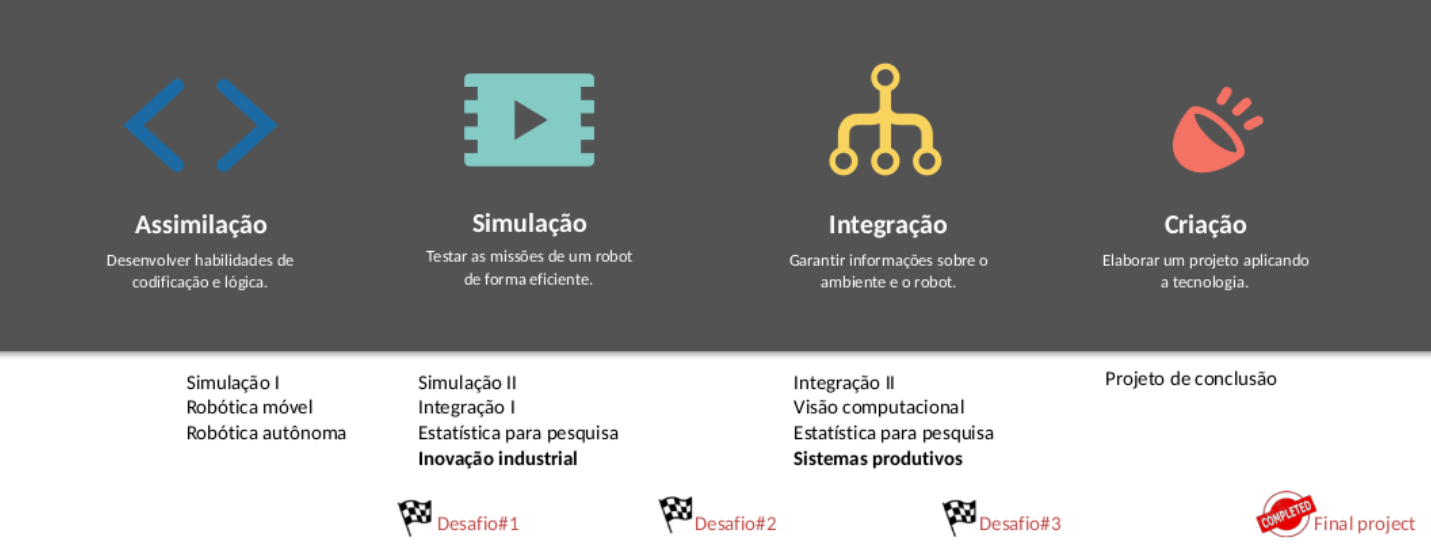
\includegraphics[width= \textwidth]{Figures/metodologia.png}
    \caption*{Fonte: Programa de Formação em Robótica e Sistemas Autônomos}
    \label{fig:metodologia}
\end{figure}

Com uma abordagem inovadora, o programa tenta realçar a busca por um aprendizado mais real e excitante para isso o conceito de professor facilitador que estimule a experiência nas várias tecnologias se faz necessário. Isso promoverá vários feedbacks mais intensos aos estudantes. Em resumo o professor será o facilitador de uma experiência de aprendizado, criando recursos e experiência para a formação do aprendiz.

% Nas próximas seções estarão descritos os materiais e métodos aplicados para cada projeto realizado durante o curso de formação em Robótica e Sistemas Autônomos. 

%\section{Desafio 1.0}
%\label{sec:met_desafio1}
%Este desafio foi feito individualmente, e ele foi realizado com o objetivo de programar o robô da \textit{Clearpath Robotics- Husky}, no ambiente de simulação do \textit{Gazebo}. A área de operação desse robô foi a área externa entre os prédios do CIMATEC 3 e 4. O \textit{Husky} tinha como missão explorar esse ambiente externo a procura de uma bola amarela, e ao identificar esta ele deveria ir até ela e parar de frente para mesma informando que a missão foi completada. Como nesse desafio foi realizada apenas a simulação, apenas o computador foi utilizado.  

%--------- NEW SECTION ----------------------
% \section{Manipulador TIMON-HM- Desafio 2.0}
% \label{sec:met_desafio2}
% O segundo desafio foi realizado em grupo, onde um manipulador deveria ser concebido desde sua fase inicial modelando toda sua estrutura e posteriormente realizada a simulação deste no \textit{Gazebo}, com a missão da câmera integrada ao manipulador identificar o \textit{tag ArUco} na caixa e pressionar o botão. Este desafio também foi realizada apenas a simulação, por isso apenas o computador foi utilizado.  

% %--------- NEW SECTION ----------------------
% \section{Manipulador Robótico JeRoTIMON- Desafio 2.2 }
% \label{sec:met_desafio2_2}
% Este desafio foi para construir o modelo real do manipulador JeRoTIMON modelado e simulado no desafio \ref{sec:met_desafio2}, realizado em grupo, onde o objetivo era o mesmo, reconhecer a \textit{tag ArUco} na caixa e pressionar o botão, só que dessa vez no ambiente real. Os materiais utilizados nesse desafio foram perfis de alumínio, motores \textit{Dynamixel}, câmera RGB modelo \textit{Teledyne Genie Nano C2590},  peças modeladas no \textit{OnShape} e impressas em \textit{ABS} por uma impressora 3D, conexões para alimentação e para comunicação

% %--------- NEW SECTION ----------------------
% \section{TIMON- HM- Desafio 2.5}
% \label{sec:met_desafio2_5}
% O desafio 2.5 foi realizado em equipe, a mesma do desafio \ref{sec:met_desafio2}, onde o robô programado foi o \textit{Darwin-OP} e este deveria realizar duas missões, a primeira, é a marcha, onde quatro robôs \textit{Darwin-OP} deveriam andar de forma sincronizada de um ponto a outro da pista de corrida. E a segunda missão foi realizada a programação para que os quatro robôs realizassem a corrida com revezamento, onde cada robô está posicionado numa parte específica da pista de corrida e ao chegar próximo um do outro eles mantém por um período a movimentação sincronizada depois o anterior para e o outro segue, igualmente a uma corrida com revezamento real.


% %--------- NEW SECTION ----------------------
% \section{UGV SACI: Integrado com Detecção Visual e Manipulador- Desafio 3.0}
% \label{sec:met_desafio3}
% Neste desafio foi desenvolvido o Saci, que integra o veículo autônomo da \textit{Clearpath Robotics Warthog} equipado com sensores (câmeras, LiDAR e GPS) e o manipulador robótico JeRoTIMON, com o propósito de transformá-lo em um robô autônomo. Este foi construído com o intuito de que o mesmo tivesse navegação autônoma para realizar investigação em ambiente externo e construir um mapa deste ambiente, detectasse a "bomba" escondida, e realizasse o desarme da bomba através do manipulador. 
% Esse projeto foi desenvolvido em duas etapas, a de simulação, onde foram utilizados o software  \textit{Gazebo} e a ferramenta de visualização \textit{Rviz}, e para configuração do pacote de parâmetros do manipulador foi utilizado \textit{MoveIt}. E em paralelo foi desenvolvido este robô em sua versão real, onde foi possível realizar testes e verificar seu desempenho em campo.



% \section{Analíse estatística R\&R da simulação do robô Darwin OP}
% \label{sec:met_analise_darwin}
% Teve como objetivo analisar o sistema de medição dos dados coletados durante os testes realizados nas etapas: de marcha e de revezamento do Desafio 2.5 (\ref{sec:met_desafio2_5}), utilizando o método de análise de variância (ANOVA). Nessa análise foi possível aplicar os conhecimentos obtidos em estatística, utilizando a ferramenta e linguagem de programação \textit{R} em um projeto realizado durante o curso, a fim de verificar o desempenho desse projeto, exemplo, a análise de precisão produzida através do estudo R\&R (Repetibilidade e Reprodutibilidade). Foram utilizadas apenas as ferramentas de simulação e para realização do estudo estatístico.


% \section{Planejamento de Experimentos (DOE) -Helicóptero de Papel (TIMON-HM)}
% \label{sec:met_analise_doe}
% Esse experimento teve como objetivo aplicar os conceitos de Planejamento de Experimento- \textit{DOE}, a um modelo de helicóptero de papel. O propósito principal foi identificar quais são os fatores que mais influenciam seu tempo de voo e como estas variáveis podem melhorar o seu desempenho. Durante o processo, foi utilizado um modelo de helicóptero em papel onde foi medido o seu tempo de voo em duas alturas diferentes, além disto, foram adicionados adesivos e um clipe em sua estrutura a fim de verificar a influência da variação destes parâmetros no resultado final. Esse estudo proporcionou a aplicação do aprendizado adquirido ao uso da ferramenta e linguagem R usada para manipulação, análise e visualização de dados, e dos conhecimentos de Estatística. 

% \section{Artigo publicado TRIS: Thermal Remote Identification System of Feverish People }
% \label{sec:met_tris}

% Esse artigo, que possui também um sistema real de mesmo nome \textit{(TRIS)}, foi modelado a partir da necessidade exposta pela pandemia do COVID-19, para identificar pessoas  foram usadas câmeras (RGB e Infravermelho), um computador para utilizar uma rede neural, e que identificasse pessoas com temperatura acima de 37,8 $^\circ$C, e informasse que aquela pessoa em questão era objeto de interesse pois estaria com febre, ou estado febril, que é um dos sintomas do COVID-19. Esse sistema foi criado com o próposito de realizar o controle da propagação do vírus. Nesse projeto puderam ser desenvolvidos os conhecimentos de rede neural, interface de sistemas, utilização de câmeras RGB e Infravermelho, e a como acontece a evolução de um projeto.